\chapter{Introduction}
\label{cha:1}

\section{Overview}

This thesis project is part of an Advanced Master of Artificial Intelligence programme—Speech and Language Technology, conducted in collaboration with the Media Bias Group \cite{media-bias-group}, who provided the topic and additional guidance along the project.

\section{Motivation and Goals}

Media bias is widespread in today's landscape, particularly on matters such as health, climate, and politics \cite{suarez-2021-prevalence-health-misinformation,wang-2024-health-misinformation,fleming-2023-climate-disinformation,tiedemann-2024-misinformation-democracy}. The existence of media bias in news sources can and has been used as a way to shape and influence public opinion \cite{aires-2020-information}. The advent of social media has exacerbated the spread of misinformation, allowing false information to easily and rapidly circulate  while remain unchecked \cite{froehlich-2024-misinformation}. For instance, a survey by \cite{allcott-2017-fake-news-election} indicated that fake news on social media played a significant role in the election of President Trump in 2016. During the COVID-19 pandemic, numerous conspiracy theories gained widespread traction through the media, with substantial support from large groups of people. A 2020 Harvard survey revealed that nearly 20\% of people believed the pandemic was a ploy "to install tracking devices inside our bodies" \cite{enders-2020-covid19-misinformation}. Despite being a major societal issue, research on the spread of misinformation on social media platforms remains scarce \cite{muhammed-2022-disaster-of-misinformation}.

\begin{figure}[htbp]
    \centering
    \fbox{
        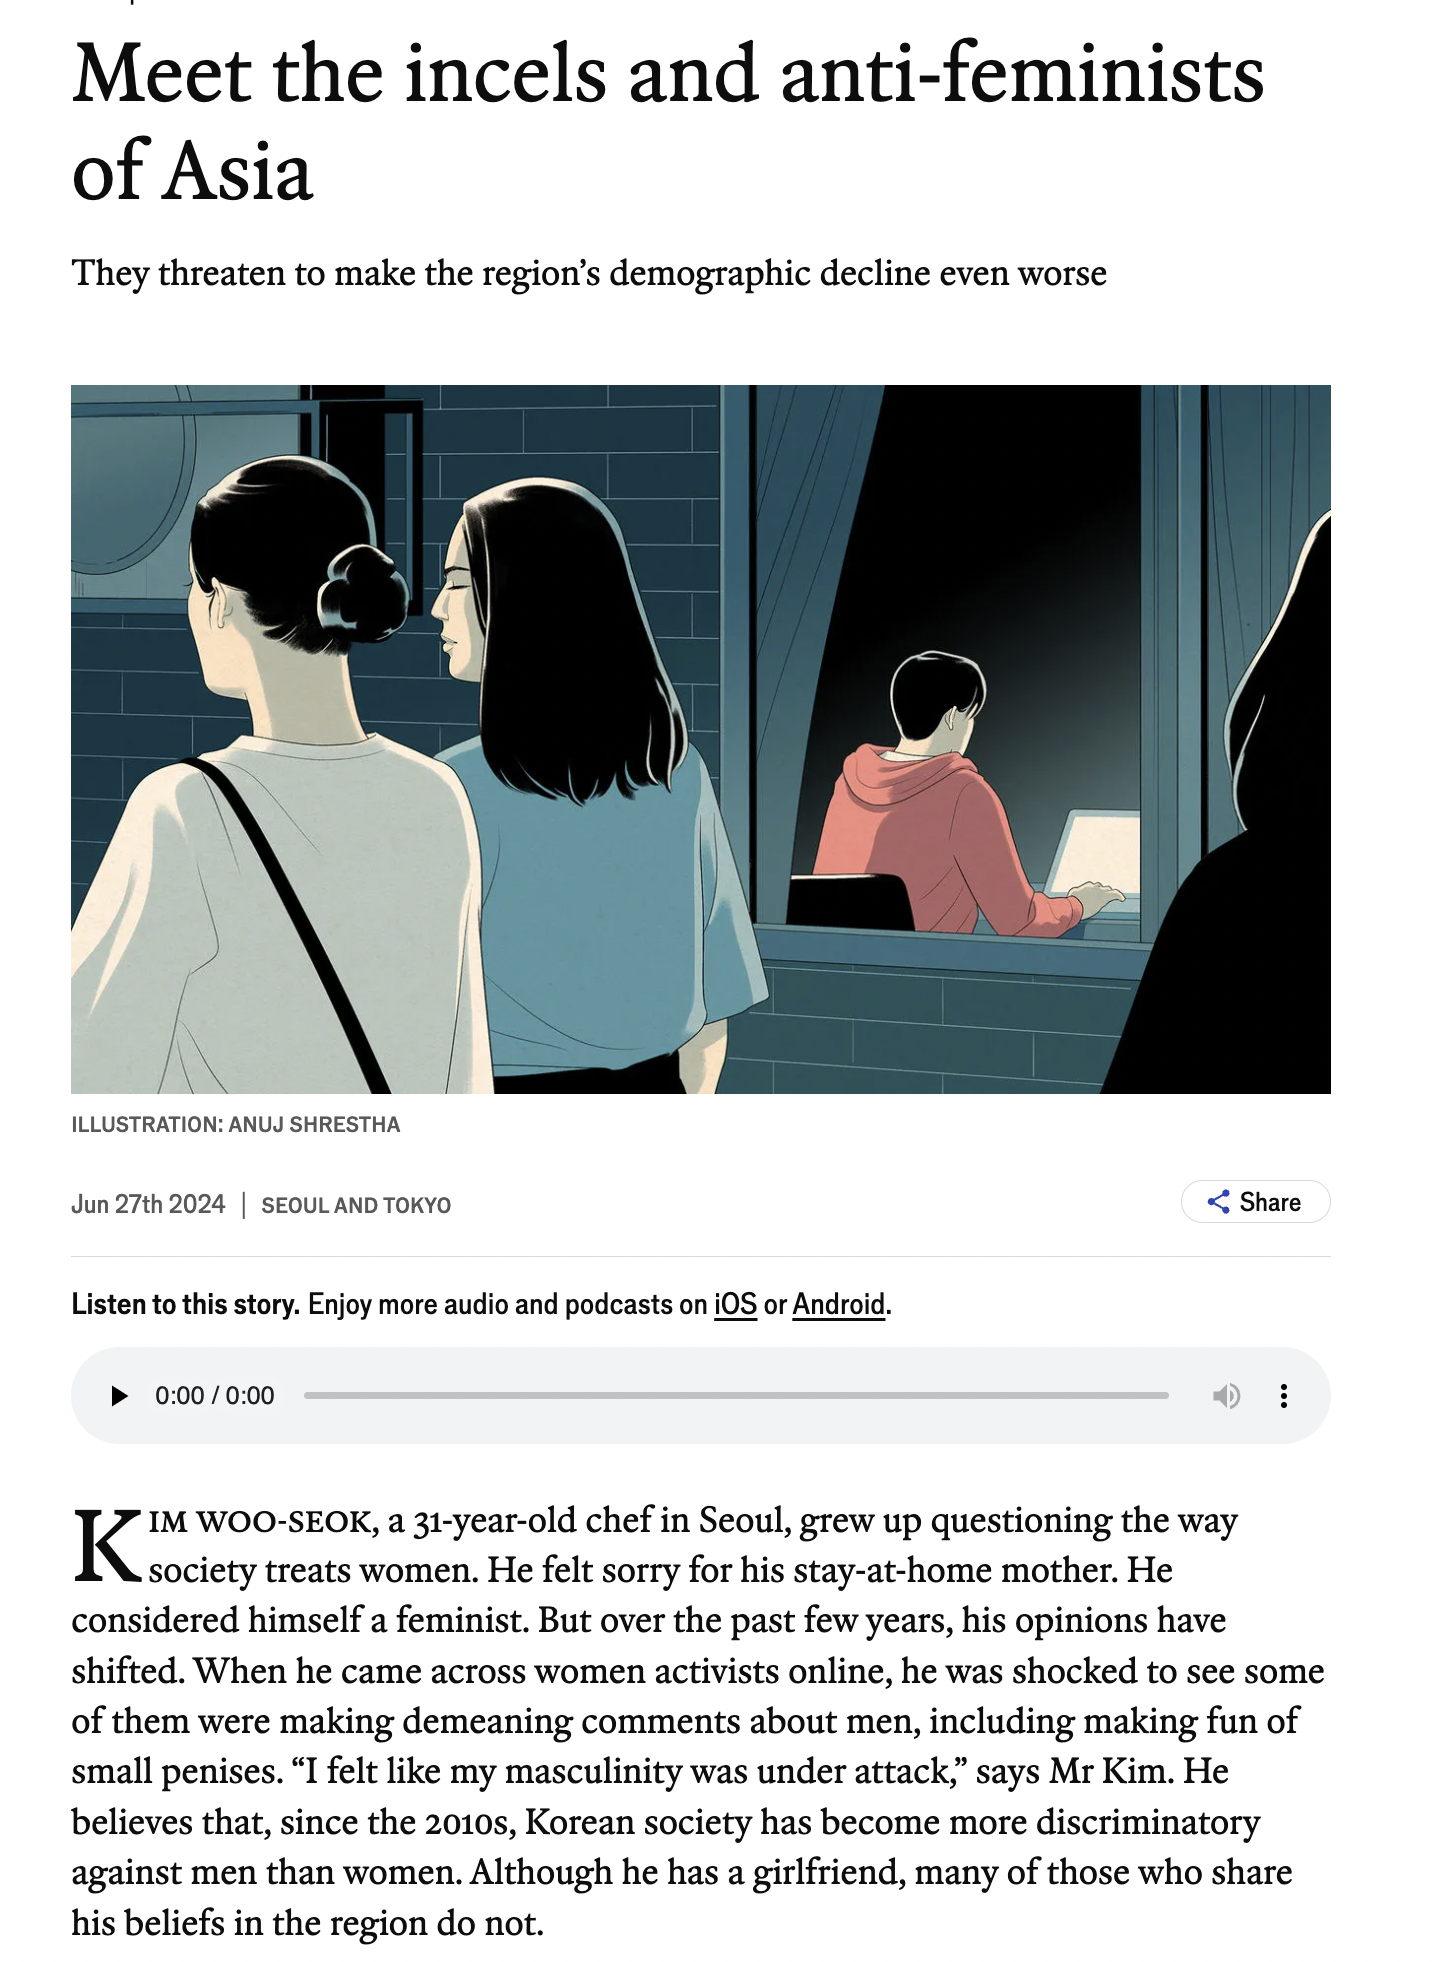
\includegraphics[width=0.7\linewidth]{images/the-economist-biased-article.png}}
    \caption{A recent article from The Economist \cite{economist-2024-incels} portraying gender discrimination with a negative-framing headline}
    \label{fig:the-economist-biased-article}
\end{figure}

An example of a biased article can be seen from a recent article published by The Economist \cite{economist-2024-incels} in Figure \ref{fig:the-economist-biased-article}. The headline includes a negative framing of certain groups, which can influence readers' perceptions before they even read the article, suggesting that the existence of these groups is inherently problematic and harmful. Terms like "incels" (involuntary celibates) and "anti-feminists" carry strong negative connotations, which can evoke emotional responses and suggest a negative view of the groups mentioned.

Ideally, unbiased media content that objectively and fairly represents multiple or a range of perspectives is desirable, news sources should remain neutral and let readers build their own opinions on the subject \cite{reuters-2021-digital-news-report}. However, this is often unachievable due to human capabilities and resource limitations; journalists cannot possibly possess complete knowledge on every topic, be physically present everywhere, or interview every relevant individual on a significant subject \cite{allsides-2022-bias-definition}. Truth and journalism objectivity is a complex matter full of choices and dilemmas, where ultimately it falls on the journalists' own preferences and criteria \cite{boudana-2011-journalistic-objectivity}. Therefore, instead of eliminating media bias, our goal should be to draw attention to its existence and forms, giving readers awareness of such content \cite{spinde-2024-taxonomy}, ultimately building a tool to defend readers from media manipulation, political agenda or indoctrination. This is essential to ensure that readers are able to form their own choices and opinions with utmost honesty and transparency.

While there exist organisations consisting of expert annotators that manually read and review articles \cite{adfontes, allsides, mbfc}, there is a growing need for more efficient methods of media bias detection. Automatic media bias detection offers a promising alternative, as developing robust systems could enhance scalability and consistency in identifying biases across a vast array of articles, addressing the limitations of manual review processes. However, this field remains relatively new, under-resourced, and challenging, due to the lack of a universally accepted definition of bias and its subtlety, which can make it difficult to identify \cite{rodrigo-2024-systematic-review-media-bias}.

Available media bias datasets \cite{spinde-2021-babe,fan-2019-basil,chen-2020-nlpcss,spinde-2023-bat,gruppi-2023-nelagt2022} are either limited in size or contain low-level, ambiguous annotations. In addition, these datasets vary in format, cover different sets of topics, contain different types of bias, and, more importantly, use different labelling formats, making it particularly difficult to compare and evaluate different media bias datasets and models trained on them. There is a critical need to develop new, richer datasets that are more extensive and varied, preferably covering a broader array of events and domains \cite{rodrigo-2024-systematic-review-media-bias}.

Existing works in media bias classification tend to have major drawbacks \cite{maab-2023-lexical-bias-detection, maab-2023-target-aware, guo-2022-modeling, van-den-berg-2020-context,lee-2021-unifying,lei-2022-sentence,lei-2024-event-relation}.
The classification is mostly done on the sentence-level with binary output, which is far too naive and may miss the broader context and impact conveyed by an entire article. Sentence-level classifiers tend to rely on low-level lexical information, which is proven to fail at the article-level \cite{chen-2020-detecting-media-bias-gaussian}. Moreover, different sentences within the same article can exhibit contradictory or varying biases. This can introduce inconsistencies and misinterpretations of the article, making it challenging to understand the article's overall bias or perspective. Media content is typically presented in the form of articles composed of multiple paragraphs, making article-level media bias classification significantly more valuable as it allows for a comprehensive understanding of the overall narrative and agenda presented by the article.

Therefore, the primary goal of this project is to develop an effective media bias classifier that encompass entire articles. This will aid readers to recognise potential biases in the information they consume, increase awareness of the dangers associated with media bias, promote media literacy, and enhance critical thinking skills, thereby enabling individuals to navigate information effectively in today's complex media landscape. To achieve this, the project will address the following research questions:
\begin{enumerate}
    \item How can current media bias datasets be improved to better support article-level classification?
    \item What are the most effective methods to represent articles and preserve contextual information for media bias classification task?
    \item How can an effective article-level media bias classifier be trained and evaluated?
    \item What are the challenges and limitations of article-level bias classification, and how can they be mitigated?
\end{enumerate}

\section{About the Media Bias Group}

The Media Bias Group \cite{media-bias-group} was established in mid-2020 by Timo Spinde during his pursuit of a Ph.D. in computer science, having been integrated into the topic since his undergraduate studies, with a vision to aid others perceive news in a more balanced and conscious manner. After a year of planning how a system could uncover bias on a vast scale encompassing millions of articles, he founded the group and forged connections with various partners, particularly those relevant to specific aspects of the project. In just one year, the project has garnered support from multiple other research groups, with around twenty students from seven countries joining to contribute to the system. Since 2021, the group has also begun offering its first Ph.D. positions.

The group is comprised of a collective of scholars across various fields such as Psychology, Linguistics, and Computer Science, with a shared goal to comprehend the factors influencing human perception of news content as biased or one-sided. Currently, the network includes six main researchers and coordinators, twenty-one professors and postdocs, as well as eight active students. Numerous publications related to media bias have been published through the network into major conferences such as EMNLP 2021 \cite{spinde-2021-babe}, along with dataset and benchmark creations.


%%% Local Variables: 
%%% mode: latex
%%% TeX-master: "thesis"
%%% End: 